\section[Анализ предметной области]{АНАЛИЗ ПРЕДМЕТНОЙ ОБЛАСТИ}

\subsection{Награды и премии Республики Беларусь}

\paragraph{}
Государственные награды Республики Беларусь представляют собой
высшую форму поощрения граждан Республики Беларусь, иностранных граждан,
лиц без гражданства, признания их вклада в защиту и укрепление государства,
приумножение экономического и духовного потенциала страны~\cite{bel_orders}.

Законодательство о государственных наградах Республики Беларусь основывается
на Конституции Республики Беларусь и состоит из закона
<<О государственных наградах Республики Беларусь>> и актов законодательства
Республики Беларусь, регулирующих отношения в данной области.

Решение о награждении государственными наградами Республики Беларусь
принимает Президент Республики Беларусь.
Оформляется такое решение указами Президента Республики Беларусь.

Присвоение звания <<Герой Беларуси>>, почетных званий Республики Беларусь,
награждение орденами и медалями Республики Беларусь производятся
в торжественной обстановке.

Государственная награда Республики Беларусь передается награжденному лично.
Вручает государственные награды Республики Беларусь
Президент Республики Беларусь либо другие должностные лица по его поручению. 

\paragraph{}
В Республике Беларусь установлены следующие государственные награды:

\begin{itemize}
\item высшая степень отличия --- звание <<Герой Беларуси>>;
\item ордена Республики Беларусь;
\item медали Республики Беларусь;
\item почетные звания Республики Беларусь.
\end{itemize}

В следующих подразделах каждый вид государственных наград
рассмотрен более подробно. 

\pagebreak
\subsection{Звание <<Герой Беларуси>>}

\paragraph{}
\textit{Звание <<Герой Беларуси>>} --- высшая степень отличия и 
государственная награда Республики Беларусь за исключительные заслуги
перед государством и обществом, связанные с подвигом,
совершенным во имя свободы, независимости и процветания Республики Беларусь.

Звание введено Законом <<О государственных наградах Республики Беларусь>>
от 13.04.1995. Звание присваивается Президентом Республики Беларусь
только один раз. Награждение может быть произведено посмертно.
Героем Беларуси могут стать не только граждане Беларуси,
но и иностранные граждане или лица без гражданства.

\paragraph{}
Лицам, удостоенным звания <<Герой Беларуси>>, 
вручается знак особого отличия --- медаль Героя Беларуси,
фотография которой приведена на рисунке~\ref{fig:medal_hero_belarus}.

\begin{figure}[h]
  \centering
  {
    \setlength{\fboxsep}{0pt}%
    \setlength{\fboxrule}{1pt}%
    \fbox{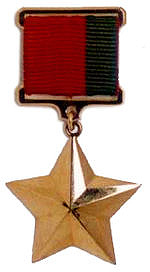
\includegraphics[width=100mm]{pic/medal_hero_belarus.jpg}}
  }
  \caption{Медаль <<Герой Беларуси>>}
  \label{fig:medal_hero_belarus}
\end{figure}

В настоящее время звания <<Герой Беларуси>> удостоены 11 граждан
Республики Беларусь.

\subsection{Ордена Республики Беларусь}

\paragraph{}
\textit{Ордена Республики Беларусь} --- почетные государственные награды
за особые заслуги в социально-экономической,
общественной и других сферах деятельности,
направленной на укрепление могущества страны, за отвагу и мужество,
проявленные при защите государства.

Приведем список орденов Республики Беларусь:
\begin{itemize}
\item орден Отечества;
\item орден Воинской славы;
\item орден <<За службу родине>>;
\item орден <<За личное мужество>>;
\item орден Дружбы народов;
\item орден Почета;
\item орден Франциска Скорины;
\item орден Матери.
\end{itemize}

\paragraph{}
Рассмотрим более подробно описание Ордена Отечества с целью установить 
характерные особенности, присущие орденам как классу государственных наград.

\textit{Орден Отечества} является высшим орденом Республики Беларусь и
имеет три степени:

\begin{itemize}
\item орден Отечества I степени;
\item орден Отечества II степени;
\item орден Отечества III степени.
\end{itemize}

Высшей степенью ордена Отечества является I степень.
Награждение производится последовательно орденом Отечества III, II и I степени:

\begin{itemize}
\item 
  за отличные достижения в производственной, научно-исследовательской,
  социально-культурной, общественной, благотворительной и иных сферах
  деятельности, направленной на повышение благосостояния людей и укрепление
  могущества страны;
\item
  за мужество и отвагу, проявленные при защите Отечества и его
  государственных интересов, обеспечении законности и правопорядка;
\item
  за большие заслуги в развитии экономических,
  научно-технических и культурных связей между Республикой Беларусь
  и другими странами.
\end{itemize}

Фотография ордена Отечества приведена на рисунке~\ref{fig:order_fatherland}.

\begin{figure}[h]
  \centering
  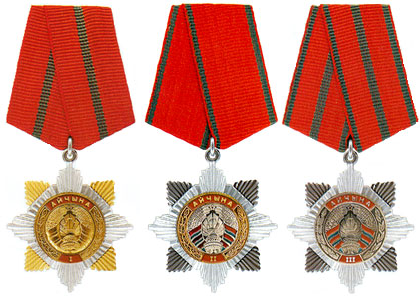
\includegraphics[width=150mm]{pic/order_fatherland.png}
  \caption{Орден Отечества}
  \label{fig:order_fatherland}
\end{figure}

Крайнее левое положение занимает орден Отечества I степени,
орден II степени расположен по центру, 
орден Отечества III степени находится в правой части изображения.


\subsection{Медали Республики Беларусь}

\paragraph{}
\textit{Медали Республики Беларусь} --- почетные государственные награды за
значительные заслуги в общественной, трудовой и других сферах деятельности
по укреплению страны, за смелые и находчивые действия,
совершенные при защите государства, охране общественного порядка.

Перечислим медали Республики Беларусь:
\begin{itemize}
\item медаль <<За отвагу>>;
\item медаль <<За отличие в воинской службе>>;
\item медаль <<За отличие в охране общественного порядка>>;
\item медаль <<За отличие в охране государственной границы>>;
\item медаль <<За отличие в предупреждении и ликвидации чрезвычайных ситуаций>>;
\item медаль <<За трудовые заслуги>>;
\item медаль Франциска Скорины;
\item медаль <<За безупречную службу>>.
\end{itemize}


\paragraph{}
Рассмотрим характерного <<представителя>> класса 
медалей --- медаль <<За отвагу>> c целью выяснить 
характерные особенности наград данного класса.

\textit{Медалью <<За отвагу>>} награждаются военнослужащие, 
лица начальствующего и рядового состава органов внутренних дел,
органов финансовых расследований Комитета государственного контроля
Республики Беларусь, органов и подразделений по чрезвычайным ситуациям
и другие граждане за личное мужество и отвагу, проявленные: 

\begin{itemize}
\item
  в боевой обстановке при защите Отечества и его государственных интересов; 
\item
  при исполнении воинского долга, служебной или гражданской обязанности,
  защите конституционных прав граждан; 
\item
  при спасении людей на воде, во время стихийных бедствий, пожаров, аварий,
  катастроф и других чрезвычайных обстоятельств, сопряженных с риском для жизни. 
\end{itemize}

Фотография медали приведена на рисунке~\ref{fig:medal_otvaga}.

\begin{figure}[h]
  \centering
  {
    \setlength{\fboxsep}{0pt}%
    \setlength{\fboxrule}{1pt}%
    \fbox{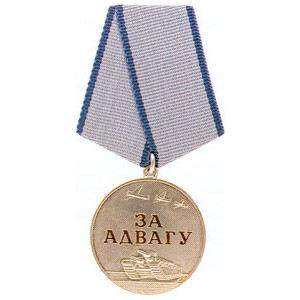
\includegraphics[width=100mm]{pic/medal_otvaga.jpg}}
  }
  \caption{Медаль <<За отвагу>>}
  \label{fig:medal_otvaga}
\end{figure}

\subsection{Почетные звания Республики Беларусь}

\paragraph{}
\textit{Почетные звания Республики Беларусь} --- это форма награды,
признания заслуг и поощрения выдающихся деятелей труда, науки, искусства,
социальной сферы, физической культуры и спорта, военного дела.
Cписок почетных званий содержит более сорока наименований.

\paragraph{}
Приведем описание одного из почетных званий с целью выяснить
характерные особенности данного класса наград.

\textit{Почетное звание <<Заслуженный тренер Республики Беларусь>>}
присваивается:

\begin{itemize}
\item
  тренерам национальных (сборных) команд Республики Беларусь,
  имеющим стаж работы с этими командами не менее четырех лет,
  --- за непосредственную подготовку и успешное выступление этих команд
  на Олимпийских играх, чемпионатах, первенствах и Кубках мира и Европы;
\item
  первым тренерам спортсменов, достигших отличных успехов
  на Олимпийских играх, чемпионатах, первенствах и Кубках мира и Европы,
  работающим с этими спортсменами не менее двух лет начиная
  с учебно-тренировочного этапа;
\item
  тренерам спортивных школ и организаций, ранее принимавшим
  непосредственное участие в подготовке переданных в высшее
  звено спортсменов, при условии работы с ними не менее четырех лет.
\end{itemize}

Фотография нагрудного знака, 
который вручается вместе с данным почетным званием, 
приведена на рисунке~\ref{fig:trener_belarus}.

\begin{figure}[h]
  \centering
  {
    \setlength{\fboxsep}{0pt}%
    \setlength{\fboxrule}{1pt}%
    \fbox{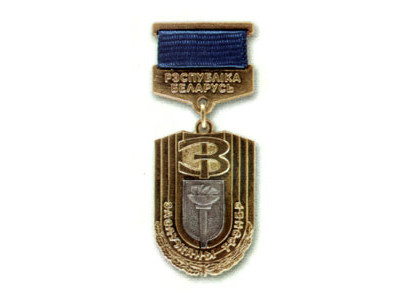
\includegraphics[width=80mm]{pic/trener_belarus.jpg}}
  }
  \caption{Нагрудный знак \\ <<Заслуженный тренер Республики Беларусь>>}
  \label{fig:trener_belarus}
\end{figure}


\subsection{Постановка задачи}

Необходимо выполнить проектирование и реализацию веб-сайта, 
способного выполнять нижеперечисленные операции:

\begin{itemize}
\item загрузка данных о наградах и награжденных из файлов
  в машиночитаемом формате;
\item обработка и представление данных о наградах и награжденных
  в виде html-страниц;
\item редактирование данных о наградах и награжденных 
  через веб-интерфейс;
\item выгрузка данных о награжденных в машиночитаемом 
  формате.
\end{itemize}

Разработанный веб-ресурс должен развертываться на платфоме,
удовлетворяющей следующим системным требованиям.

Аппаратные требования:
\begin{itemize}
\item Intel-совместимый процессор с частотой не менее 1 Ггц;
\item полнодуплексное подключение к сети Интернет с
  пропускной способностью не менее 10 МБ/с;
\item объем оперативной памяти не менее 512 МБ.
\end{itemize}

Программные требования:
\begin{itemize}
\item работа сервера должна производиться на *nix-совместимой 
  операционной системе;
\item в качестве хранилища данных должна использоваться 
  СУБД реляционного типа;
\item программное обеспечение, которое будет использоваться при 
  развертывании веб-ресурса, должно быть открытым и (или) распространяться 
  на бесплатной основе для некоммерчекого использования. 
\end{itemize}

Кроме этого, необходимо выполнить проектирование базы данных, 
способной эффективно хранить данные предметной области, а также
разработать руководство по использованию разработанного сервиса.